\chapter{Phân tích và thiết kế hệ thống Yoca}
\label{Chapter3}

Chương này trình bày quá trình phân tích và thiết kế hệ thống Yoca, nền tảng web hỗ trợ phân tích dữ liệu on-chain, dữ liệu thị trường và hành vi ví blockchain. Tiếp nối bối cảnh và mục tiêu đã nêu ở Chương 1 cùng các hệ thống liên quan và cơ sở công nghệ đã trình bày ở Chương 2, Chương 3 tập trung làm rõ cách hệ thống Yoca được tổ chức để hiện thực hóa các mục tiêu đó, bao gồm ý tưởng ứng dụng, các tình huống sử dụng tiêu biểu, yêu cầu chức năng và phi chức năng, kiến trúc tổng thể, các luồng nghiệp vụ cốt lõi và định hướng thiết kế cơ sở dữ liệu. Do đề tài thuộc nhóm ứng dụng, chương chỉ tập trung vào các thành phần trọng tâm và các quyết định thiết kế quan trọng, không đi sâu mô tả toàn bộ chi tiết cài đặt hay toàn bộ bảng dữ liệu.

Yoca được xây dựng theo hướng ứng dụng web full-stack, trong đó frontend đảm nhiệm trình bày giao diện và trực quan hóa dữ liệu, còn backend đảm nhiệm xác thực, xử lý nghiệp vụ, tích hợp và chuẩn hóa dữ liệu từ bên thứ ba. Vì phải làm việc với dữ liệu blockchain có khối lượng lớn, biến động liên tục và phụ thuộc vào nhiều nhà cung cấp API, hệ thống cần có chiến lược truy xuất, lưu trữ đệm và đồng bộ dữ liệu hợp lý để đảm bảo khả năng phản hồi, ổn định và mở rộng.


Nhóm chúng em tổ chức các chức năng thành một hành trình phân tích liền mạch. Người dùng có thể bắt đầu ở Market Overview để nhận biết token hoặc pool đáng chú ý, mở Pool Detail để xem thanh khoản và giao dịch, rồi chuyển đến Token Overview để đọc dữ liệu thị trường, holder và lịch sử biến động. Khi một địa chỉ ví xuất hiện trong quá trình tìm hiểu, Wallet Overview tiếp tục cung cấp danh mục, lịch sử hoạt động, PnL và các biểu đồ liên quan. Nếu muốn theo dõi lâu dài, người dùng đăng nhập để lưu ví hoặc token, đặt nhãn, cấu hình cảnh báo và sử dụng AI để diễn giải tập dữ liệu đã chọn.

Yoca được phát triển với định hướng trở thành một nền tảng phân tích dữ liệu crypto và wallet intelligence, giúp người dùng theo dõi thị trường, phân tích token, quan sát hoạt động ví và khai thác các tín hiệu on-chain trong cùng một giao diện thống nhất. Trong bối cảnh thị trường blockchain phát triển nhanh, dữ liệu liên quan đến token, ví, giao dịch, dòng tiền và tin tức thường bị phân tán trên nhiều công cụ khác nhau. Người dùng muốn có một bức tranh đầy đủ thường phải tra cứu nhiều nguồn, đối chiếu dữ liệu thủ công và tự diễn giải các biểu đồ hoặc lịch sử giao dịch. Quá trình này tốn thời gian, dễ sai sót và gây khó khăn đối với người dùng chưa có nhiều kinh nghiệm phân tích dữ liệu on-chain.

Ngoài luồng chính, Yoca còn hỗ trợ so sánh nhiều ví, xem chi tiết giao dịch và phân tích dấu hiệu wash trading. Đây là các nhánh dành cho người dùng cần đi sâu hơn sau bước quan sát tổng quan. Mô-đun wash trading trình bày quan hệ ví--giao dịch dưới dạng đồ thị và các chỉ số bất thường; kết quả đóng vai trò tín hiệu để người dùng tiếp tục kiểm tra giao dịch cùng bối cảnh thị trường.

Tình huống sử dụng đầu tiên là phân tích một ví blockchain. Người dùng nhập địa chỉ ví vào hệ thống để xem tổng quan danh mục, các token đang nắm giữ, giá trị ước tính, lịch sử giao dịch và các biểu đồ biến động theo thời gian. Thay vì đọc từng giao dịch riêng lẻ trên trình khám phá khối, người dùng có thể quan sát ví thông qua các góc nhìn tổng hợp như phân bổ tài sản, biến động số dư, số lượng giao dịch và các hoạt động swap đáng chú ý. Tình huống này đặc biệt hữu ích khi người dùng muốn hiểu một ví đang có xu hướng nắm giữ dài hạn, giao dịch thường xuyên hay thay đổi danh mục theo biến động thị trường.

Từ hành trình trên, yêu cầu của Yoca được gom thành sáu nhóm theo năng lực mà người dùng nhận được.

Tình huống sử dụng thứ ba là so sánh và đánh giá nhiều ví. Đối với người dùng có nhu cầu theo dõi nhiều địa chỉ ví, hệ thống hỗ trợ quan sát và đối chiếu các chỉ số ở cấp độ ví. Người dùng có thể so sánh danh mục, mức độ hoạt động, hiệu suất và các dấu hiệu hành vi giữa các ví khác nhau. Đây là tình huống có giá trị đối với nhà nghiên cứu token, nhà phân tích ví hoặc người dùng muốn theo dõi các ví có ảnh hưởng trong hệ sinh thái.

Tình huống sử dụng thứ tư là thiết lập cảnh báo. Người dùng đã đăng nhập có thể cấu hình các cảnh báo liên quan đến token hoặc ví. Khi một điều kiện được thỏa mãn, chẳng hạn biến động giá, hoạt động ví hoặc một sự kiện đáng chú ý, hệ thống ghi nhận và hỗ trợ thông báo cho người dùng. Chức năng này làm giảm nhu cầu theo dõi thủ công liên tục, đồng thời giúp người dùng phản ứng nhanh hơn với các thay đổi quan trọng.

Tình huống sử dụng thứ năm là sử dụng AI để hỗ trợ diễn giải dữ liệu. Dữ liệu on-chain thường có nhiều trường kỹ thuật và không dễ đọc đối với người dùng phổ thông. Vì vậy, Yoca định hướng tích hợp trợ lý AI nhằm tóm tắt dữ liệu ví, giải thích các biến động nổi bật và hỗ trợ người dùng đặt câu hỏi trên dữ liệu đã được hệ thống chuẩn hóa. Trong thiết kế này, AI không thay thế các phép tính định lượng của hệ thống, mà đóng vai trò như một lớp hỗ trợ diễn giải kết quả bằng ngôn ngữ tự nhiên.


Chức năng so sánh nhiều ví sử dụng cùng các khái niệm ở cấp độ tổng hợp. Người dùng có thể chọn nhiều địa chỉ và đặt các chỉ số chính cạnh nhau để đối chiếu giá trị danh mục, PnL, win rate và hoạt động giao dịch. Với dữ liệu không đủ độ phủ, giao diện thể hiện rõ phạm vi của kết quả để người dùng không nhầm phần dữ liệu hiện có với toàn bộ lịch sử.

Dựa trên mục tiêu đề tài và các tình huống sử dụng đã nêu, hệ thống Yoca được phân tích theo hai nhóm yêu cầu chính: yêu cầu chức năng và yêu cầu phi chức năng. Yêu cầu chức năng mô tả những nghiệp vụ mà hệ thống cần hỗ trợ cho người dùng, trong khi yêu cầu phi chức năng mô tả các thuộc tính chất lượng như hiệu năng, bảo mật, tính ổn định, khả năng mở rộng và khả năng sử dụng.

Yoca cần cho phép người dùng chọn token hoặc dữ liệu giao dịch phù hợp để quan sát các mẫu đáng chú ý như chu trình chuyển tài sản, cấu trúc tập trung quanh một số ví và khối lượng tương đối của từng ví trong tập giao dịch. Hệ thống trình bày kết quả bằng đồ thị, bảng và phần giải thích để người dùng có thể lần ngược về các ví hoặc giao dịch liên quan. Các tín hiệu phải được diễn đạt theo mức độ nghi vấn; hệ thống không được tự động đồng nhất một mẫu bất thường với kết luận gian lận.

Về yêu cầu chức năng, nhóm yêu cầu đầu tiên là quản lý tài khoản và xác thực người dùng. Hệ thống cần hỗ trợ đăng ký, đăng nhập, duy trì phiên làm việc và xác thực các thao tác yêu cầu quyền truy cập cá nhân hóa. Các chức năng như quản lý hồ sơ, watchlist, tag ví, cảnh báo và gói đăng ký chỉ nên được sử dụng bởi người dùng đã xác thực. Bên cạnh đăng nhập bằng tài khoản thông thường, hệ thống cũng hỗ trợ các hướng xác thực phù hợp với sản phẩm blockchain như đăng nhập thông qua ví.

Nhóm yêu cầu thứ hai là phân tích thị trường và token. Hệ thống cần cho phép người dùng tìm kiếm token, xem danh sách token, xem thông tin chi tiết token, dữ liệu giá, biểu đồ lịch sử và các chỉ số liên quan đến thị trường. Các dữ liệu này được lấy từ các nguồn bên thứ ba, sau đó được backend chuẩn hóa và trả về cho frontend dưới dạng phù hợp với bảng dữ liệu hoặc biểu đồ. Đây là nhóm chức năng tạo nền tảng để người dùng hiểu bối cảnh thị trường trước khi phân tích sâu hơn ở cấp độ ví.

Nhóm yêu cầu thứ ba là phân tích ví. Đây là một trong những nhóm chức năng trọng tâm của Yoca. Hệ thống cần cho phép người dùng nhập địa chỉ ví để xem tổng quan ví, danh mục token, lịch sử giao dịch, lịch sử chuyển tài sản, lịch sử swap, biến động số dư và hiệu suất theo thời gian. Đối với các ví có nhiều giao dịch, hệ thống cần có cơ chế phân trang, lưu trữ đệm và tái sử dụng dữ liệu để tránh việc phải truy xuất lại toàn bộ lịch sử từ nhà cung cấp bên ngoài trong mỗi lần người dùng mở trang.

Nhóm yêu cầu thứ tư là trực quan hóa dữ liệu. Hệ thống cần chuyển các dữ liệu đã xử lý thành biểu đồ dễ đọc, bao gồm biểu đồ giá token, biểu đồ giá trị danh mục, biểu đồ số dư, biểu đồ phân bổ tài sản, biểu đồ giao dịch và các biểu đồ hỗ trợ so sánh. Trực quan hóa không chỉ phục vụ mục đích trình bày mà còn là phương tiện chính giúp người dùng nhận diện xu hướng, biến động và các điểm bất thường trong dữ liệu.

Nhóm yêu cầu thứ năm là AI-assisted analysis và wallet chat. Hệ thống cần hỗ trợ chuyển dữ liệu ví hoặc dữ liệu token đã được xử lý thành ngữ cảnh có cấu trúc, sau đó sử dụng mô hình AI để tạo phần tóm tắt hoặc trả lời câu hỏi của người dùng. Kết quả AI cần được trình bày như một dạng hỗ trợ phân tích, không phải là kết luận tài chính tuyệt đối. Khi phù hợp, hệ thống có thể lưu lại kết quả phân tích để tránh lặp lại các tác vụ tốn chi phí và cải thiện tốc độ phản hồi trong các lần truy vấn sau.

Hệ thống lưu lịch sử thông báo theo tài khoản, hỗ trợ trạng thái đã đọc/chưa đọc và dùng khóa sự kiện để tránh tạo bản ghi trùng khi webhook gửi lại cùng một hoạt động. Các cơ chế này giúp người dùng theo dõi kết quả gửi cảnh báo và duy trì lịch sử nhất quán.

Nhóm yêu cầu thứ bảy là quản lý hồ sơ, watchlist, nhãn ví và gói dịch vụ. Người dùng cần có khả năng lưu lại token hoặc ví quan tâm, gắn nhãn cho ví, quản lý thông tin cá nhân và theo dõi trạng thái gói đăng ký. Các chức năng này giúp hệ thống không chỉ là một công cụ tra cứu một lần, mà trở thành một không gian làm việc cá nhân hóa cho hoạt động phân tích dữ liệu blockchain.

Về yêu cầu phi chức năng, yêu cầu đầu tiên là hiệu năng. Do hệ thống phải làm việc với dữ liệu có khối lượng lớn và phụ thuộc vào nhiều API bên ngoài, backend cần ưu tiên đọc dữ liệu đã cache trước khi gọi lại nhà cung cấp. Đối với các dữ liệu có tần suất truy cập cao như dữ liệu token, dữ liệu biểu đồ hoặc dữ liệu lịch sử ví, cơ chế cache đóng vai trò quan trọng trong việc giảm độ trễ và giảm nguy cơ bị giới hạn tần suất truy vấn.

Do mỗi lần gọi mô hình phát sinh chi phí, hệ thống theo dõi lượt dùng theo tài khoản và gói dịch vụ. Khi vượt quyền lợi, người dùng nhận được thông báo rõ ràng cùng đường dẫn đến thông tin gói phù hợp.

Yêu cầu phi chức năng thứ ba là bảo mật. Các chức năng liên quan đến tài khoản, watchlist, tag ví, cảnh báo, thanh toán và hồ sơ người dùng cần được bảo vệ bởi cơ chế xác thực và phân quyền. Token xác thực cần được quản lý an toàn, các API nhận dữ liệu từ người dùng cần được kiểm tra đầu vào, và các cấu hình nhạy cảm như API key, secret thanh toán hoặc secret xác thực không được đưa trực tiếp vào mã nguồn phía client.

Yêu cầu phi chức năng thứ tư là khả năng mở rộng. Mặc dù hệ thống hiện tập trung nhiều vào Solana, thiết kế cần đủ linh hoạt để có thể mở rộng sang các nguồn dữ liệu hoặc blockchain khác. Điều này đòi hỏi backend phải tách biệt logic nghiệp vụ với logic tích hợp từng provider. Khi cần bổ sung provider mới, hệ thống nên chỉ cần thêm adapter hoặc service tương ứng thay vì phải sửa trực tiếp nhiều phần giao diện và nghiệp vụ.

Yêu cầu thứ hai là khả năng phản hồi trong điều kiện phụ thuộc API bên ngoài. Hệ thống tái sử dụng dữ liệu còn hiệu lực, chỉ đồng bộ khoảng lịch sử còn thiếu và thể hiện trạng thái tải ở từng khu vực. Những yêu cầu trùng nhau phát sinh đồng thời được dùng chung kết quả đang xử lý, qua đó giảm số lần gọi provider và giữ giao diện phản hồi theo từng thành phần.

\subsection{Sơ đồ Use Case tổng quát}

% Sơ đồ use case tổng quát mô tả các tác nhân chính và nhóm chức năng lớn của hệ thống Yoca. Trong phạm vi thiết kế, hệ thống có bốn nhóm tác nhân chính: người dùng chưa đăng nhập, người dùng đã đăng nhập, quản trị viên và các dịch vụ bên thứ ba. Người dùng chưa đăng nhập có thể tra cứu một số thông tin công khai như thị trường, token hoặc ví. Người dùng đã đăng nhập có thể sử dụng các chức năng cá nhân hóa như quản lý watchlist, gắn nhãn ví, tạo cảnh báo, xem hồ sơ và sử dụng các chức năng yêu cầu xác thực. Quản trị viên có thể theo dõi, cấu hình hoặc quản lý một số dữ liệu hệ thống tùy theo phạm vi triển khai. Các dịch vụ bên thứ ba cung cấp dữ liệu blockchain, dữ liệu thị trường, AI, thanh toán và webhook.

Yêu cầu cuối cùng là khả năng sử dụng và bảo trì. Một người dùng mới cần tìm được token hoặc ví, hiểu trạng thái loading/error/empty và đọc được các chỉ số chính mà không phải biết cấu trúc API. Các màn hình cốt lõi cần dùng thuật ngữ, màu sắc và hành vi component nhất quán. Khi chuyển giữa tiếng Việt và tiếng Anh, hệ thống phải thay đổi đồng bộ chuỗi giao diện, định dạng số, ngày giờ và đơn vị tiền tệ; giá trị gốc bằng USD chỉ được quy đổi sang VND tại lớp trình bày để không làm thay đổi dữ liệu nghiệp vụ. Ở phía phát triển, contract dữ liệu giữa client và server phải đủ rõ để thay đổi provider không buộc giao diện phụ thuộc vào response thô của từng dịch vụ.

\section{Sơ đồ Use Case}
\label{sec:use_case}

Sơ đồ tổng quát trong Hình~\ref{fig:usecase} mô tả hai tác nhân Khách và Người dùng đã đăng ký. Người dùng đã đăng ký kế thừa các chức năng công khai của Khách, đồng thời có thêm những chức năng cần dữ liệu cá nhân hoặc phát sinh chi phí như quản lý tài khoản, cảnh báo, subscription và AI. Provider, webhook và cổng thanh toán là các hệ thống hỗ trợ phía sau nên được trình bày trong sơ đồ kiến trúc, tách khỏi các tác nhân sử dụng Yoca.

\begin{figure}[H]
    \centering
    \includegraphics[width=0.8\textwidth]{images/usecase.png}
    \caption{Sơ đồ Use-case của hệ thống Yoca}
    \label{fig:usecase}
\end{figure}

Hình~\ref{fig:usecase_guest} triển khai chi tiết những điểm vào công khai: trang chủ, Market Radar, tìm kiếm, chi tiết token và chi tiết ví. Pool, giao dịch và các nhánh phân tích sâu được truy cập từ những điểm vào này, giúp sơ đồ tập trung vào mục tiêu chính của khách.

Yoca được tổ chức theo kiến trúc ứng dụng web full-stack, gồm hai ứng dụng chính là frontend và backend. Frontend được xây dựng bằng React và Vite, có nhiệm vụ hiển thị giao diện, nhận thao tác người dùng, gọi API và trực quan hóa dữ liệu. Backend được xây dựng bằng Hono, có nhiệm vụ định nghĩa API, xác thực yêu cầu, xử lý nghiệp vụ, truy cập cơ sở dữ liệu và tích hợp với các nhà cung cấp dữ liệu bên ngoài. Cơ sở dữ liệu PostgreSQL được sử dụng để lưu trữ dữ liệu người dùng, dữ liệu cache, metadata, lịch sử cảnh báo, dữ liệu thanh toán và các kết quả phân tích cần tái sử dụng.

Ở mức tổng thể, một yêu cầu từ người dùng thường đi qua các bước chính. Đầu tiên, người dùng thao tác trên một trang hoặc một component của frontend. Sau đó, frontend gọi một client service tương ứng để gửi yêu cầu đến backend. Backend tiếp nhận yêu cầu thông qua route, kiểm tra xác thực nếu cần, kiểm tra dữ liệu đầu vào và gọi domain service phù hợp. Domain service sẽ ưu tiên đọc dữ liệu trong PostgreSQL nếu dữ liệu đã được cache và còn phù hợp. Nếu dữ liệu chưa có hoặc đã quá cũ, service sẽ gọi nhà cung cấp bên ngoài, chuẩn hóa kết quả, lưu lại vào cơ sở dữ liệu và trả dữ liệu về cho frontend. Cuối cùng, frontend sử dụng dữ liệu này để hiển thị bảng, biểu đồ, báo cáo, cảnh báo hoặc phần trình bày từ AI.


% TODO: Bổ sung sơ đồ kiến trúc tổng thể.
\begin{figure}[H]
    \centering
    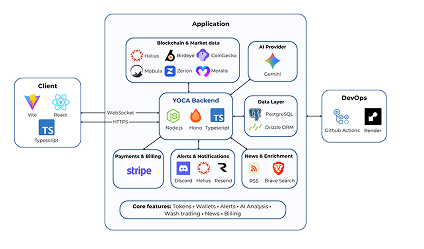
\includegraphics[width=1\textwidth]{images/arch.jpg}
    \caption{Kiến trúc tổng thể của hệ thống Yoca}
    \label{fig:kien_truc_tong_the}
\end{figure}

% Hình~\ref{fig:kien_truc_tong_the} nên thể hiện các thành phần chính gồm React frontend, Hono API backend, PostgreSQL, các domain service, các provider bên ngoài như Helius, Moralis, CoinGecko, Birdeye, Google Gemini, Stripe và Solana RPC. Ngoài ra, sơ đồ cũng nên làm rõ hướng dữ liệu đi từ frontend đến backend, từ backend đến cache, từ backend đến provider, sau đó quay lại frontend dưới dạng dữ liệu đã chuẩn hóa.


\subsection{Kiến trúc Monolith phân lớp và cơ chế Tải dữ liệu động (Lazy Loading)}

Trong phạm vi triển khai hiện tại, backend của Yoca được tổ chức theo hướng monolith phân lớp. Điều này có nghĩa là hệ thống backend được triển khai như một ứng dụng API thống nhất, nhưng bên trong được chia thành các lớp và miền nghiệp vụ riêng biệt. Các route chịu trách nhiệm tiếp nhận HTTP request và trả response. Các service chịu trách nhiệm xử lý nghiệp vụ. Các module tích hợp provider chịu trách nhiệm gọi API bên ngoài và chuẩn hóa dữ liệu. Lớp cơ sở dữ liệu chịu trách nhiệm định nghĩa schema, truy vấn và lưu trữ dữ liệu.

Cách tổ chức này phù hợp với quy mô của đồ án vì giúp hệ thống dễ triển khai, dễ kiểm thử và dễ theo dõi hơn so với việc tách thành nhiều microservices độc lập ngay từ đầu. Khi phát triển một sản phẩm có nhiều miền dữ liệu như token, ví, biểu đồ, AI, cảnh báo, thanh toán và hồ sơ người dùng, việc chia backend thành nhiều service vật lý có thể làm tăng độ phức tạp vận hành. Ngược lại, monolith phân lớp giúp nhóm tập trung vào việc hoàn thiện nghiệp vụ, đồng thời vẫn duy trì được cấu trúc module rõ ràng để có thể tách nhỏ trong tương lai nếu hệ thống phát triển lớn hơn.

Ở phía frontend, cơ chế tải dữ liệu động được áp dụng theo tương tác và ngữ cảnh sử dụng của người dùng. Thay vì tải toàn bộ dữ liệu ngay khi người dùng mở ứng dụng, mỗi trang hoặc thành phần giao diện chỉ gọi dữ liệu cần thiết cho chức năng hiện tại. Ví dụ, trang market chỉ cần dữ liệu thị trường và danh sách token, trang chi tiết token cần thêm dữ liệu lịch sử và biểu đồ, trong khi trang ví cần dữ liệu danh mục, giao dịch và lịch sử số dư. Cách tiếp cận này giúp giảm lượng dữ liệu tải ban đầu, cải thiện trải nghiệm người dùng và hạn chế số lượt gọi API không cần thiết.

Cơ chế tải dữ liệu động cũng phù hợp với đặc thù của dữ liệu blockchain. Một ví có thể có lịch sử giao dịch rất dài, nhưng người dùng không phải lúc nào cũng cần xem toàn bộ lịch sử đó ngay lập tức. Hệ thống có thể tải trước phần tổng quan, sau đó tải các phần chi tiết như giao dịch, swap hoặc biểu đồ số dư khi người dùng mở tab tương ứng. Cách làm này giúp phân bổ chi phí truy vấn theo nhu cầu thực tế, tránh gây tải lớn cho backend và provider bên ngoài.

\subsection{Chiến lược lưu trữ đệm (Caching) đa tầng}
% Rất quan trọng: Giải thích cơ chế TTL/window filtering cho dữ liệu ví, và on-conflict upserts cho dữ liệu thị trường (Token market/chart caches).

Caching là một trong những quyết định thiết kế quan trọng của Yoca. Dữ liệu on-chain và dữ liệu thị trường thường được lấy từ các nhà cung cấp bên thứ ba, trong khi các nhà cung cấp này có thể áp dụng giới hạn tần suất truy vấn, giới hạn gói sử dụng hoặc thay đổi độ trễ theo thời điểm. Nếu mỗi lần người dùng mở một trang hoặc thay đổi bộ lọc hệ thống đều gọi trực tiếp provider, ứng dụng sẽ dễ gặp lỗi rate limit, phản hồi chậm và khó kiểm soát chi phí. Vì vậy, hệ thống cần lưu trữ đệm dữ liệu đã lấy và tái sử dụng trong những trường hợp phù hợp.

Chiến lược caching của Yoca được thiết kế theo hướng ưu tiên cơ sở dữ liệu. Đối với các dữ liệu có thể tái sử dụng như lịch sử ví, danh mục tài sản, giao dịch, chuyển token, swap, dữ liệu biểu đồ và dữ liệu token, backend sẽ kiểm tra dữ liệu trong PostgreSQL trước. Nếu dữ liệu đã tồn tại và còn nằm trong ngưỡng hợp lệ, hệ thống trả về dữ liệu cache. Nếu dữ liệu chưa có hoặc không còn đủ mới, hệ thống gọi provider bên ngoài để đồng bộ phần dữ liệu cần thiết, sau đó chuẩn hóa và lưu lại vào cơ sở dữ liệu.

Đối với dữ liệu ví, caching cần quan tâm đến khái niệm khoảng thời gian dữ liệu đã được đồng bộ. Một ví có thể đã được đồng bộ lịch sử giao dịch cho một giai đoạn nhất định, nhưng chưa đầy đủ ở một giai đoạn khác. Vì vậy, hệ thống cần sử dụng metadata hoặc thông tin coverage để phân biệt phần dữ liệu đã có và phần dữ liệu còn thiếu. Cách tiếp cận này giúp hệ thống không phải tải lại toàn bộ lịch sử ví mỗi lần người dùng truy vấn, đồng thời vẫn đảm bảo khả năng bổ sung dữ liệu mới khi cần.

Đối với dữ liệu token và dữ liệu thị trường, hệ thống có thể sử dụng cơ chế TTL và ngưỡng cập nhật. Dữ liệu thị trường gần thời gian thực cần được cập nhật thường xuyên hơn, trong khi dữ liệu lịch sử cũ có thể được tái sử dụng lâu hơn. Khi nhận dữ liệu mới, backend có thể thực hiện upsert để cập nhật hoặc bổ sung bản ghi mà không tạo dữ liệu trùng lặp. Cách tiếp cận này giúp duy trì tập dữ liệu rolling ổn định cho các biểu đồ và bảng thống kê.

Caching không chỉ phục vụ hiệu năng mà còn giúp hệ thống ổn định hơn. Khi provider bên ngoài gặp lỗi tạm thời, dữ liệu cache có thể được sử dụng như một phương án dự phòng nếu vẫn còn phù hợp. Điều này đặc biệt quan trọng đối với các trang phân tích ví và biểu đồ, vì người dùng thường kỳ vọng hệ thống vẫn hiển thị được dữ liệu đã truy xuất trước đó thay vì báo lỗi hoàn toàn khi provider không phản hồi.



\subsection{Cơ chế đồng bộ hóa dữ liệu từ các nhà cung cấp (Helius, CoinGecko)}

Yoca tích hợp nhiều nhà cung cấp dữ liệu để phục vụ các miền nghiệp vụ khác nhau. Đối với dữ liệu ví Solana, hệ thống sử dụng Helius để truy xuất danh mục, lịch sử giao dịch, chuyển token và swap. Đối với dữ liệu thị trường và dữ liệu lịch sử giá token, hệ thống sử dụng CoinGecko. Ngoài ra, hệ thống còn có các đường tích hợp khác như Moralis cho một số luồng dữ liệu EVM hoặc dữ liệu dự phòng, Birdeye như một hướng fallback hoặc legacy path cho một số dữ liệu token, Google Gemini cho AI-assisted analysis, Stripe cho thanh toán và Solana RPC hoặc Helius RPC cho xác minh thanh toán on-chain.

Việc đồng bộ dữ liệu từ nhiều provider đòi hỏi backend phải có lớp chuẩn hóa dữ liệu. Mỗi provider có định dạng phản hồi, giới hạn truy vấn và cách biểu diễn dữ liệu khác nhau. Nếu frontend hoặc domain service phụ thuộc trực tiếp vào dữ liệu thô từ provider, hệ thống sẽ khó bảo trì và dễ bị ảnh hưởng khi provider thay đổi. Vì vậy, Yoca sử dụng các adapter hoặc service chuyên biệt để gọi provider, chuyển dữ liệu về DTO nội bộ và chỉ trả về định dạng đã được chuẩn hóa cho các lớp phía trên.

Đối với dữ liệu ví, luồng đồng bộ thường bắt đầu bằng việc người dùng nhập địa chỉ ví hoặc mở lại một ví đã từng phân tích. Backend kiểm tra metadata cache để xác định dữ liệu đã có. Nếu dữ liệu thiếu hoặc cần cập nhật, backend gọi provider để lấy dữ liệu mới theo từng loại như portfolio, transactions, transfers hoặc swaps. Sau đó, dữ liệu được chuẩn hóa, lưu vào các bảng cache tương ứng và trả về cho frontend. Cách tiếp cận này giúp hệ thống quản lý dữ liệu ví theo từng miền nhỏ thay vì xử lý toàn bộ dữ liệu ví như một khối đơn lẻ.

Đối với dữ liệu token, backend cần ánh xạ token address sang định danh phù hợp với nguồn dữ liệu giá. Đây là bước quan trọng vì mỗi provider có thể dùng khóa định danh khác nhau. Sau khi ánh xạ được token, hệ thống có thể lấy dữ liệu thị trường, dữ liệu giá lịch sử hoặc dữ liệu biểu đồ. Các dữ liệu này sau đó được lưu lại để phục vụ các lần truy vấn tiếp theo.

Cơ chế đồng bộ cũng cần xử lý lỗi và giới hạn truy vấn. Khi provider trả về lỗi 429 hoặc lỗi tạm thời, hệ thống cần có chính sách chờ, retry hoặc trả về dữ liệu cache nếu có. Khi nhiều API key được cấu hình, hệ thống có thể xoay vòng key để giảm nguy cơ gián đoạn. Những cơ chế này giúp hệ thống hoạt động ổn định hơn trong điều kiện phụ thuộc vào nhiều dịch vụ bên ngoài.



\section{Thiết kế chi tiết các luồng nghiệp vụ cốt lõi (Sequence Diagrams)}
\label{sec:thiet_ke_luong_nghiep_vu}

Phần này trình bày ba luồng nghiệp vụ cốt lõi của hệ thống: truy xuất và tổng hợp lịch sử giao dịch ví, truy vấn và trực quan hóa dữ liệu biểu đồ, và vấn đáp dữ liệu thông qua AI Assistant. Các luồng này đại diện cho những vấn đề kỹ thuật chính của Yoca, bao gồm truy xuất dữ liệu on-chain, sử dụng cache, chuẩn hóa dữ liệu, hiển thị biểu đồ và diễn giải dữ liệu.

\subsection{Luồng truy xuất và tổng hợp lịch sử giao dịch ví}

Luồng truy xuất và tổng hợp lịch sử giao dịch ví bắt đầu khi người dùng nhập một địa chỉ ví hoặc mở trang chi tiết ví. Frontend gửi yêu cầu đến backend thông qua service tương ứng. Backend tiếp nhận yêu cầu tại route ví, kiểm tra định dạng địa chỉ, xác định loại dữ liệu cần truy xuất và gọi wallet domain service.

Wallet service trước hết kiểm tra dữ liệu cache trong PostgreSQL. Nếu hệ thống đã có dữ liệu tổng quan, danh mục và lịch sử giao dịch còn phù hợp, service sẽ đọc dữ liệu từ cache và trả về cho route. Nếu cache chưa tồn tại hoặc chưa đủ dữ liệu cho khoảng thời gian người dùng yêu cầu, service gọi lớp fetcher để truy xuất dữ liệu từ provider bên ngoài. Dữ liệu nhận được từ provider được chuẩn hóa thành định dạng nội bộ, sau đó được lưu vào các bảng cache và metadata tương ứng.

Sau khi dữ liệu đã được chuẩn hóa, backend tổng hợp các thông tin cần thiết cho frontend. Các thông tin này có thể bao gồm danh sách token trong ví, giá trị ước tính, lịch sử giao dịch, giao dịch chuyển token, hoạt động swap và các thống kê tổng quan. Frontend nhận dữ liệu trả về, cập nhật trạng thái giao diện và hiển thị dữ liệu dưới dạng bảng hoặc biểu đồ.

% % TODO: Bổ sung sequence diagram cho luồng truy xuất ví.
% \begin{figure}[htbp]
% \centering
% \fbox{
% \begin{minipage}{0.85\textwidth}
% \centering
% \vspace{1.2cm}
% Sequence Diagram: Luồng truy xuất và tổng hợp lịch sử giao dịch ví \
% \textit{TODO: Chèn sơ đồ tuần tự tại đây.}
% \vspace{1.2cm}
% \end{minipage}
% }
% \caption{Luồng truy xuất và tổng hợp lịch sử giao dịch ví}
% \label{fig:lich_su_giao_dich}
% \end{figure}

% Hình~\ref{fig:lich_su_giao_dich} nên thể hiện các thành phần chính gồm User, React Frontend, Hono Route, Wallet Service, Cache Retriever, Provider Fetcher, PostgreSQL và Helius. Điểm cần nhấn mạnh trong sơ đồ là backend không gọi provider ngay lập tức trong mọi trường hợp, mà kiểm tra cache trước, sau đó chỉ gọi provider khi dữ liệu thiếu hoặc đã hết hạn.



\subsection{Luồng truy vấn và trực quan hóa biểu đồ (Chart Data Flow)}

Luồng truy vấn dữ liệu biểu đồ bắt đầu khi người dùng mở một trang có biểu đồ hoặc thay đổi tham số như token, ví, khoảng thời gian hoặc loại biểu đồ. Frontend gọi chart API thông qua service đã định nghĩa. Request gửi lên backend chứa các thông tin cần thiết để xác định loại biểu đồ, đối tượng phân tích và khoảng thời gian cần truy vấn.

Backend tiếp nhận request tại chart route. Tùy theo loại biểu đồ, route có thể gọi chart service, token service hoặc wallet service. Ví dụ, biểu đồ lịch sử giá token sẽ dựa nhiều vào dữ liệu token và dữ liệu thị trường, trong khi biểu đồ biến động số dư ví sẽ dựa vào dữ liệu ví và dữ liệu lịch sử số dư. Service tương ứng kiểm tra cache trước, sau đó gọi provider nếu dữ liệu chưa đủ hoặc cần cập nhật.

Dữ liệu biểu đồ sau khi được lấy từ cache hoặc provider sẽ được chuẩn hóa thành chuỗi thời gian. Mỗi điểm dữ liệu cần có mốc thời gian, giá trị và các metadata cần thiết để frontend có thể hiển thị. Đối với một số biểu đồ phức tạp, chẳng hạn biểu đồ số dư theo token hoặc biểu đồ giá trị danh mục, backend có thể cần kết hợp dữ liệu giao dịch với dữ liệu giá lịch sử để tính ra giá trị tại từng thời điểm.

Frontend nhận dữ liệu đã chuẩn hóa và truyền vào các component biểu đồ. Các component này chịu trách nhiệm hiển thị trục thời gian, đường dữ liệu, tooltip, chú thích, trạng thái tải dữ liệu và trạng thái lỗi. Cách tách biệt giữa backend xử lý dữ liệu và frontend hiển thị biểu đồ giúp hệ thống dễ mở rộng thêm loại biểu đồ mới mà không làm thay đổi quá nhiều cấu trúc tổng thể.

% % TODO: Bổ sung sequence diagram cho Chart Data Flow.
% \begin{figure}[htbp]
% \centering
% \fbox{
% \begin{minipage}{0.85\textwidth}
% \centering
% \vspace{1.2cm}
% Sequence Diagram: Luồng truy vấn và trực quan hóa biểu đồ \
% \textit{TODO: Chèn sơ đồ tuần tự tại đây.}
% \vspace{1.2cm}
% \end{minipage}
% }
% \caption{Luồng truy vấn và trực quan hóa dữ liệu biểu đồ}
% \label{fig:chart_data_flow}
% \end{figure}

% Hình~\ref{fig:chart_data_flow} nên thể hiện các thành phần gồm Chart Component, Chart API Client, Hono Chart Route, Chart Service, Token hoặc Wallet Service, PostgreSQL Cache và provider như CoinGecko hoặc Helius. Điểm cốt lõi của luồng là dữ liệu biểu đồ phải được chuẩn hóa trước khi trả về frontend để đảm bảo các component biểu đồ có thể tái sử dụng.

\subsection{Luồng vấn đáp dữ liệu thông qua AI Assistant}

Luồng vấn đáp thông qua AI Assistant bắt đầu khi người dùng đặt câu hỏi hoặc yêu cầu hệ thống phân tích một ví, một token hoặc một tập dữ liệu đã hiển thị. Frontend gửi câu hỏi cùng với ngữ cảnh cần thiết đến backend. Backend kiểm tra xác thực nếu chức năng yêu cầu người dùng đăng nhập, sau đó gọi service phụ trách wallet chat hoặc AI analysis.

Trước khi gọi mô hình AI, backend cần chuẩn bị ngữ cảnh dữ liệu. Đây là bước quan trọng vì AI không nên tự tạo ra số liệu hoặc tự suy đoán dữ liệu không có trong hệ thống. Service sẽ thu thập các chỉ số đã được tính toán, dữ liệu ví đã chuẩn hóa, dữ liệu token liên quan hoặc các kết quả phân tích có sẵn. Sau đó, backend chuyển các dữ liệu này thành một ngữ cảnh có cấu trúc để gửi đến mô hình AI.

Mô hình AI sử dụng ngữ cảnh đã chuẩn bị để tạo câu trả lời bằng ngôn ngữ tự nhiên. Câu trả lời có thể bao gồm tóm tắt danh mục ví, nhận xét về biến động tài sản, các giao dịch đáng chú ý hoặc giải thích một biểu đồ nhất định. Sau khi nhận kết quả, backend có thể lưu lại câu trả lời hoặc phiên chat nếu chức năng lưu lịch sử được bật. Frontend hiển thị câu trả lời trong giao diện chat hoặc trong vùng phân tích tương ứng.

% % TODO: Bổ sung sequence diagram cho AI Assistant.
% \begin{figure}[htbp]
% \centering
% \fbox{
% \begin{minipage}{0.85\textwidth}
% \centering
% \vspace{1.2cm}
% Sequence Diagram: Luồng vấn đáp dữ liệu thông qua AI Assistant \
% \textit{TODO: Chèn sơ đồ tuần tự tại đây.}
% \vspace{1.2cm}
% \end{minipage}
% }
% \caption{Luồng vấn đáp dữ liệu thông qua AI Assistant}
% \label{fig:ai_assistant}
% \end{figure}

% Hình~\ref{fig:ai_assistant} nên thể hiện các thành phần gồm User, Chat Component, Hono Route, Wallet Chat Service, PostgreSQL, AI Provider và giao diện trả kết quả. Điểm quan trọng cần thể hiện là AI chỉ nhận dữ liệu đã được backend chuẩn hóa và tóm tắt, thay vì truy cập trực tiếp vào dữ liệu thô hoặc tự tạo ra số liệu.


\input{Chapter3/database/database}

\section{Tiêu chí chấp nhận và phạm vi kiểm thử}
\label{sec:acceptance_plan}

Nhóm chúng em xác định tiêu chí chấp nhận theo các hành trình chính của người dùng. Các tiêu chí trong Bảng~\ref{tab:acceptance_criteria} liên kết yêu cầu chức năng với hành vi cần được duy trì khi hệ thống thay đổi; kết quả chạy các suite kiểm thử được trình bày tại Chương 5.

\small
\begin{longtable}{|p{3.1cm}|p{5.4cm}|p{6.0cm}|}
\caption{Kịch bản và tiêu chí chấp nhận các luồng chính}\label{tab:acceptance_criteria} \\
\hline
\textbf{Luồng} & \textbf{Kịch bản} & \textbf{Tiêu chí chấp nhận} \\
\hline
\endfirsthead
\hline
\textbf{Luồng} & \textbf{Kịch bản} & \textbf{Tiêu chí chấp nhận} \\
\hline
\endhead

Khám phá thị trường & Mở Market Overview, tìm token/pool/ví và chuyển giữa các trang liên quan & Kết quả dẫn đến đúng đối tượng; loading, empty và upstream error được hiển thị rõ; dữ liệu chính có đơn vị và thời điểm phù hợp \\
\hline
Token và pool & Mở token, xem chart/holder/pool rồi mở một pool và giao dịch gần đây & Address được giữ nhất quán qua các trang; biểu đồ và bảng không dùng dữ liệu sai schema; trường tùy chọn bị thiếu không làm hỏng toàn trang \\
\hline
Phân tích ví & Mở ví, thay khoảng thời gian, xem portfolio, PnL, balance, transfer và swap & Dữ liệu thuộc đúng ví và khoảng thời gian; danh sách lớn được phân trang/lọc; kết quả có giới hạn độ phủ phải được ghi rõ \\
\hline
So sánh và wash trading & So sánh nhiều ví; mở phân tích wash trading của một token và lần theo giao dịch liên quan & Các chỉ số dùng cùng định nghĩa; đồ thị liên kết được với dữ liệu nguồn; tín hiệu bất thường không được trình bày như kết luận chắc chắn \\
\hline
Tài khoản cá nhân & Đăng nhập, cập nhật profile, quản lý watchlist/label và thử truy cập dữ liệu của tài khoản khác & Thao tác hợp lệ được lưu; route bảo vệ từ chối request thiếu hoặc sai quyền; dữ liệu cá nhân không bị trả cho tài khoản khác \\
\hline
Cảnh báo & Tạo, sửa trạng thái và xóa cảnh báo token hoặc ví; tiếp nhận một sự kiện phù hợp & Rule được lưu đúng chủ sở hữu và điều kiện; sự kiện phù hợp được xử lý theo kênh hỗ trợ; lỗi provider không làm mất cấu hình cảnh báo \\
\hline
AI và subscription & Gửi câu hỏi có ngữ cảnh, quản lý session/prompt và sử dụng hết quota thử nghiệm & Phản hồi bám dữ liệu được cung cấp; lượt dùng được ghi nhận; chức năng bị khóa trả thông báo và hướng nâng gói rõ ràng \\
\hline
\end{longtable}
\normalsize

Phạm vi kiểm thử gồm các phép tính và normalizer, contract bằng fixture cho phản hồi provider, route/service với upstream được mock và component test cho trạng thái giao diện. Các ca kiểm thử tập trung vào validation, ownership, phân trang, dữ liệu nullable, chống ghi trùng, quota và cách hệ thống phản hồi khi dịch vụ bên ngoài trả lỗi. Cách tổ chức này bao phủ các ranh giới có ảnh hưởng trực tiếp đến dữ liệu hiển thị và những luồng nghiệp vụ chính trong Bảng~\ref{tab:acceptance_criteria}.

\section{Tổng kết chương}

Chương này đã chuyển mục tiêu chung của Yoca thành một hành trình sử dụng và các yêu cầu có thể đối chiếu. Khách có thể khám phá thị trường, token, pool, giao dịch và ví; người dùng đã đăng ký có thêm không gian cá nhân, cảnh báo, subscription và AI. So sánh ví và wash trading mở rộng luồng phân tích khi người dùng cần đối chiếu nhiều đối tượng hoặc quan sát quan hệ giao dịch.

Bên cạnh chức năng, nhóm chúng em đặt ra yêu cầu về khả năng kiểm chứng dữ liệu, xử lý lỗi, bảo vệ dữ liệu cá nhân và tính nhất quán của giao diện. Chương tiếp theo trình bày cách kiến trúc Yoca đáp ứng các yêu cầu trên trong điều kiện dữ liệu phụ thuộc nhiều provider.
